%!TEX root = main.tex
\chapter{Design details / Implementation details}

%Here you describe a more detailed view of the various parts of the 
%architecture describing how the robot controller or game was designed.

%TODO: Pakkediagram, klassediagram, (sekvens om nødvendig)
%Generelt om implementasjonen, de ulike scenene/states, hovedaktører, scenemanagers/statemanagers, grafikk. Gameplay etc.  + mye mere jeg ikke kommer på i farta :D 

As mentioned earlier, the chosen development tools are Android SDK for this game, the natural choice when developing applications for the Android Platform. 

With Model-View Controller in mind, the different classes are seperated into model, view and controller packages. In addition, the game contains packages for listeners and states. 

\begin{figure}[ht]
    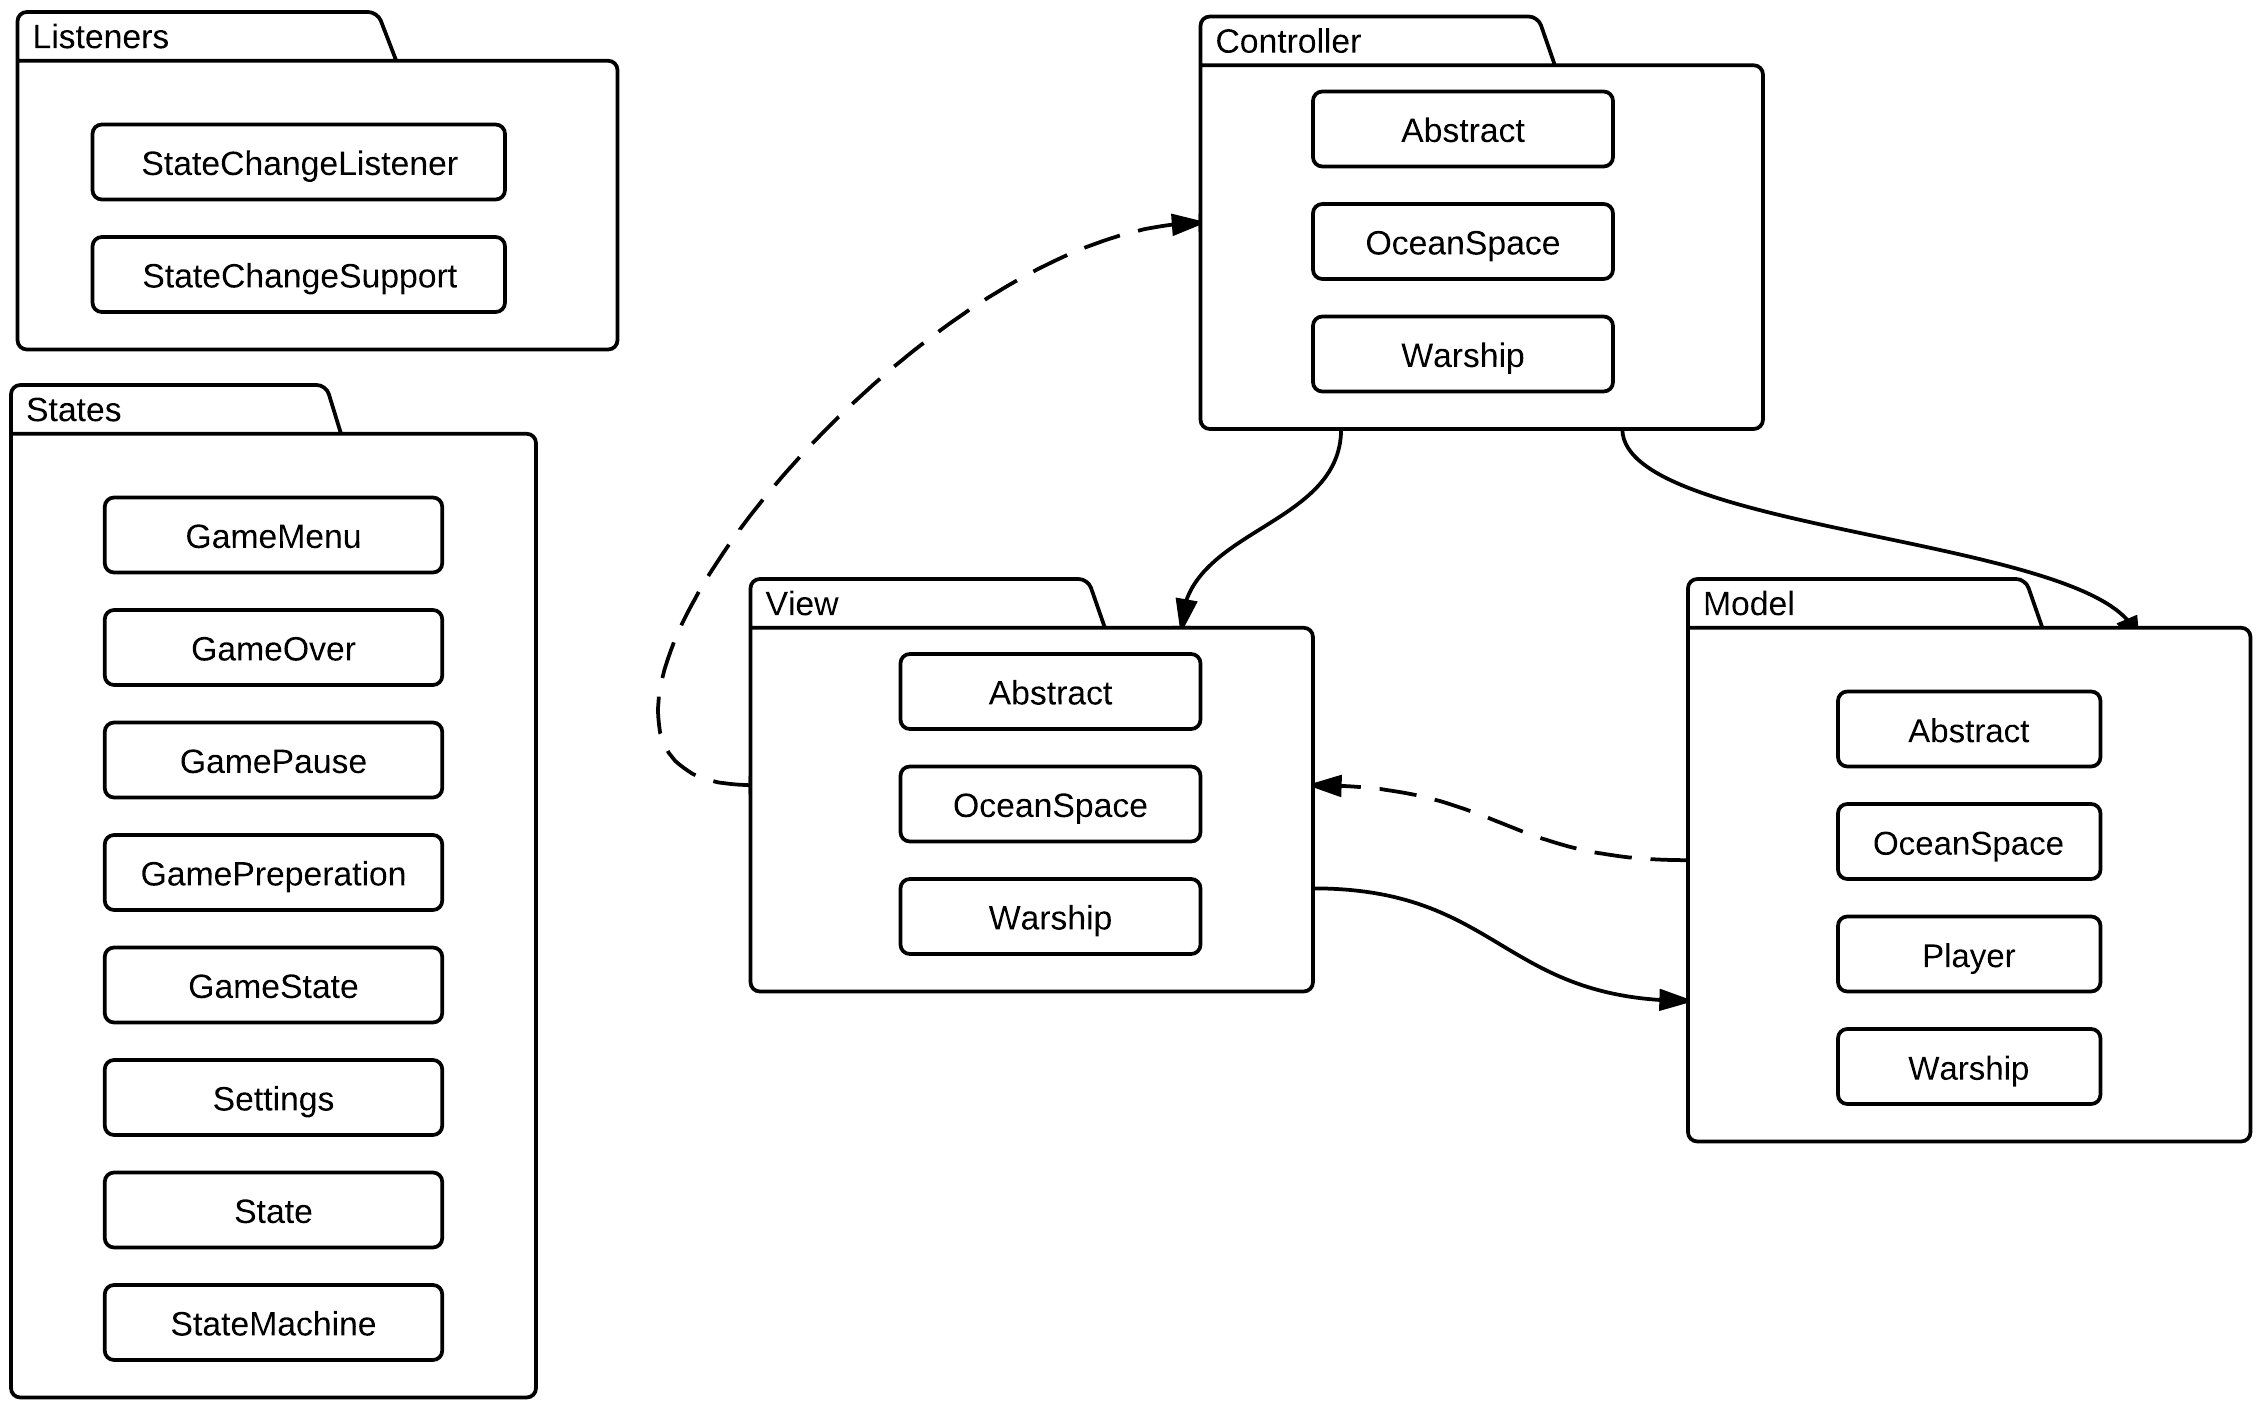
\includegraphics[width=\textwidth]{img/PackageDiagram.png}
    \caption{Package Diagram}
    \label{fig:PackageDiagram}
\end{figure}

Each package contain either models, views or controllers for warships and oceanspace. Models inherit listener methods from an abstract class called AbstractModel, while Views and Controllers inherit draw methods and controller methods. The latter provide functionality to add and remove connected views and models to a given controller. See the appendix for more detailed diagrams for models \ref{fig:ClassModel}, views \ref{fig:ClassView} and controllers \ref{fig:ClassController}.

Since the state pattern are one of the primary patterns and we didn't use any additional library or framework to support that pattern, we had to implement this by ourselves. The state package contain states for every scenario in the game; GameMenu, GameOver, GamePause, GamePreperation and GameState. GamePreperation is a state where the user does some pre-game actions, like positioning and rotating ships. Each state implement common methods from a main class called State. These methods give support for user interaction, in addition to StateMachine features. The StateMachine class functions as a controller for the different states, and stores them in a stack. One can both push and pop states to and from the stack, from within each state class. By using the state pattern, transitions between different scenarios become more effective and intuitive. For further information regarding these state classes, see \ref{fig:ClassState}, where detailed diagrams show the interaction between the classes, and which methods these classes contain.

